

Autonomous agents observe their environment, make decisions, and perform tasks with minimal human interference \citep{sutton2018reinforcement}.
These agents have been successfully evaluated across a wide range of application domains. However, developing algorithms for autonomous agents that can be deployed in real-world scenarios presents significant challenges \citep{dulac2021challenges}. These challenges include dealing with high-dimensional state and action spaces, partial observability, non-stationarity, sparse rewards, and the need for safety constraints. Furthermore, real-world environments often have multiple objectives, require sample efficiency, and necessitate robust and explainable decision-making. Addressing these challenges is crucial for productionizing reinforcement learning algorithms to real-world problems. 


\begin{table}[ht]
\footnotesize
\centering
\setlength{\tabcolsep}{3pt} % default value: 6pt
\newcommand{\cmark}{\textcolor{green!80!black}{\ding{51}}}
\newcommand{\xmark}{\textcolor{red}{\ding{55}}}
\begin{tabular}{c>{\centering}p{2.5cm}cccc>{\centering\arraybackslash}p{1.3cm}}
\toprule
\multirow{2}{*}{\textbf{Benchmark}} & \multicolumn{4}{c}{\textbf{Metrics}} & \multirow{2}{*}{\makecell{\textbf{Real-World} \\ \textbf{Tasks}}} & \multirow{2}{*}{\makecell{\textbf{Offline} \\ \textbf{Datasets}}} \\ 
\cmidrule(lr){2-5}
 & \textbf{Generalization} & \textbf{System} & \textbf{Data Cost} & \textbf{Reliability} &  & \\ 
\midrule
\method & \cmark & \cmark & \cmark & \cmark & \cmark & \cmark \\
\midrule
% D4RL \citep{fu2020d4rl} & \cmark & \xmark & \xmark & \xmark & \cmark & \cmark \\
D5RL \citep{rafailov2024d5rl} & \cmark & \xmark & \xmark & \xmark & \cmark & \cmark \\

NeoRL \citep{qin2022neorl} & \xmark & \xmark & \xmark & \xmark & \cmark & \cmark \\
OGBench \citep{park2024ogbench} & \cmark & \xmark & \xmark & \xmark & \cmark & \cmark \\
Meta-World \citep{meta_world} & \cmark & \xmark & \xmark & \xmark & \cmark & \xmark \\
% CoinRun \citep{coin_run} & \cmark & \xmark & \xmark & \xmark & \xmark & \xmark \\
DM Control \citep{tassa2018deepmind} & \xmark & \xmark & \xmark & \xmark & \xmark & \xmark \\
Jumanji \cite{bonnet2023jumanji}  & \cmark & \xmark & \xmark & \xmark & \cmark & \xmark \\
DSRL \cite{liu2023datasets}  & \xmark & \xmark & \xmark & \xmark & \cmark & \cmark \\
Safety Gym \citep{ji2023safety_gym} & \xmark & \xmark & \xmark & \cmark & \cmark & \xmark \\
ALE \citep{bellemare2013arcade} & \xmark & \xmark & \xmark & \xmark & \xmark & \xmark \\
MineRL \citep{guss2019minerl} & \cmark & \xmark & \xmark & \xmark & \xmark & \cmark \\
% OpenAI Gym \citep{brockman2016openai}  & \xmark & \xmark & \xmark & \xmark & \xmark & \xmark \\
Loon Benchmark \citep{balloon_learning_env}  & \cmark & \xmark & \xmark & \xmark & \cmark & \cmark \\ 
\bottomrule
\end{tabular}
\vspace{0.5em}
\caption{\method compared to existing benchmarks that evaluate autonomous agents. Checkmarks (\cmark) indicate the presence of a feature or metric, while crosses (\xmark) denote its absence.
\method distinguishes itself by including metrics for generalization, system resource efficiency, data cost, and reliability, in addition to providing real-world tasks and offline datasets.
Here, real-world tasks refer to those that are often performed in industrial or consumer contexts. 
The selected domains in \method are designed to closely mirror real-world challenges, ensuring the relevance and transferability of the benchmark results to practical applications. }
\label{tab:benchmark_comparison}
\vspace{-1.2em}
\end{table}


To enable researchers to develop algorithms with real-world deployment considerations in mind, there is a need for benchmarks that incorporate practical metrics. These include metrics such as the compute required for training and inference, wall-clock time, and effort expended on data collection. While there are existing benchmarks for autonomous agents \citep{guss2019minerl, meta_world, kempka2016vizdoom, bellemare2013arcade, MinigridMiniworld23, tassa2018deepmind}, most only evaluate an agent's raw performance on the same task on which it was trained, without considering numerous other metrics that matter in real-world production training and deployment scenarios.

% In this paper, we introduce \method\footnote{\method~code: \url{https://github.com/Farama-Foundation/A2Perf}, Website: \url{https://a2perf.farama.org}}, a benchmark that aims to bridge the gap between algorithms research and real-world applications by providing a comprehensive evaluation platform for autonomous agents, thereby  expanding the applicability of reinforcement learning to a wide range of practical domains.
In this paper, we introduce \method\footnote{\method~code: \url{https://anonymous.4open.science/r/A2Perf-2BFC}}, a benchmarking framework that aims to bridge the gap between algorithms research and real-world applications by providing a comprehensive evaluation platform for autonomous agents, thereby expanding the applicability of reinforcement learning to a wide range of practical domains. In addition, it comes equipped with a critical set of metrics for fair assessment.

\method incorporates three challenging domains based on prior work \citep{coumans2023motion, mirhoseini2021graph, gur2021environment} that closely mirror scenarios that have been demonstrated in the real world: computer chip-floorplanning, website form-filling and navigation, and quadruped locomotion.
In addition, these domains were chosen because they inherently exhibit a small Sim2Real gap.
The computer chip-floorplanning domain \citep{mirhoseini2020chip_placement, mirhoseini2021graph} was used to help create an iteration of Google's tensor processing unit\footnote{History of the Tensor Processing Unit: \url{https://shorturl.at/Bo71S}}, where the agent optimizes the layout of chip components.
In the website form-filling and navigation domain \citep{gur2018learning_to_navigate_the_web, gur2021environment}, agents autonomously navigate and interact with websites in a Google Chrome\footnote{Google Chrome Browser: \url{ https://www.google.com/chrome/}} browser, making it identical to real-world web navigation.
The quadruped locomotion domain \citep{peng2020learning_agile_imitate} has demonstrated successful transfer of learned walking gaits to the Unitree Laikago\footnote{Unitree Laikago: \url{https://shorturl.at/FD6uP}} robot. 

Furthermore, to address the metrics gap, \method provides an open-source benchmarking suite that evaluates agents across four key metric categories: (1) data cost, which quantifies the effort required to gather training data for imitation learning, (2) application performance, relating to the quality of the agent's task-specific execution, and its ability to generalize to tasks that it was not explicitly trained to perform; (3) system resource efficiency, focusing on the hardware resources used during training and inference; and (4) reliability, denoting the consistency of an agent's performance over training and inference. While three domains and for classes of metrics are currently available, A2Perf allows for straightforward expansion to benchmark on custom domains and for custom metrics.


The key contributions of this work include:
\begin{itemize}
\item A \textbf{unified evaluation framework} that combines critical metrics spanning data cost, system resources, reliability, and generalization, applied across three diverse domains with demonstrated real-world applicability: computer chip floorplanning, web navigation, and quadruped locomotion.
\item A novel \textbf{data cost metric} that enables fair comparisons between different learning paradigms (e.g., imitation learning vs reinforcement learning)
\item An \textbf{open-source, extensible implementation} that facilitates reproducible evaluation and community contributions
\end{itemize}
% The key contributions of this work include:
% \begin{itemize}
%     \item A \textbf{unified evaluation framework} that combines critical metrics spanning data cost, system resources, reliability, and generalization.
%     \item Three domains with \textbf{demonstrated real-world transfer}: computer chip floorplanning, web navigation, and quadruped locomotion
%     \item A novel \textbf{data cost metric} that enables fair comparisons between different learning paradigms (e.g., imitation learning vs reinforcement learning)
%     \item An open-source, extensible implementation that facilitates reproducible evaluation and community contributions
% \end{itemize}


\begin{figure}[!ht]
    \centering
    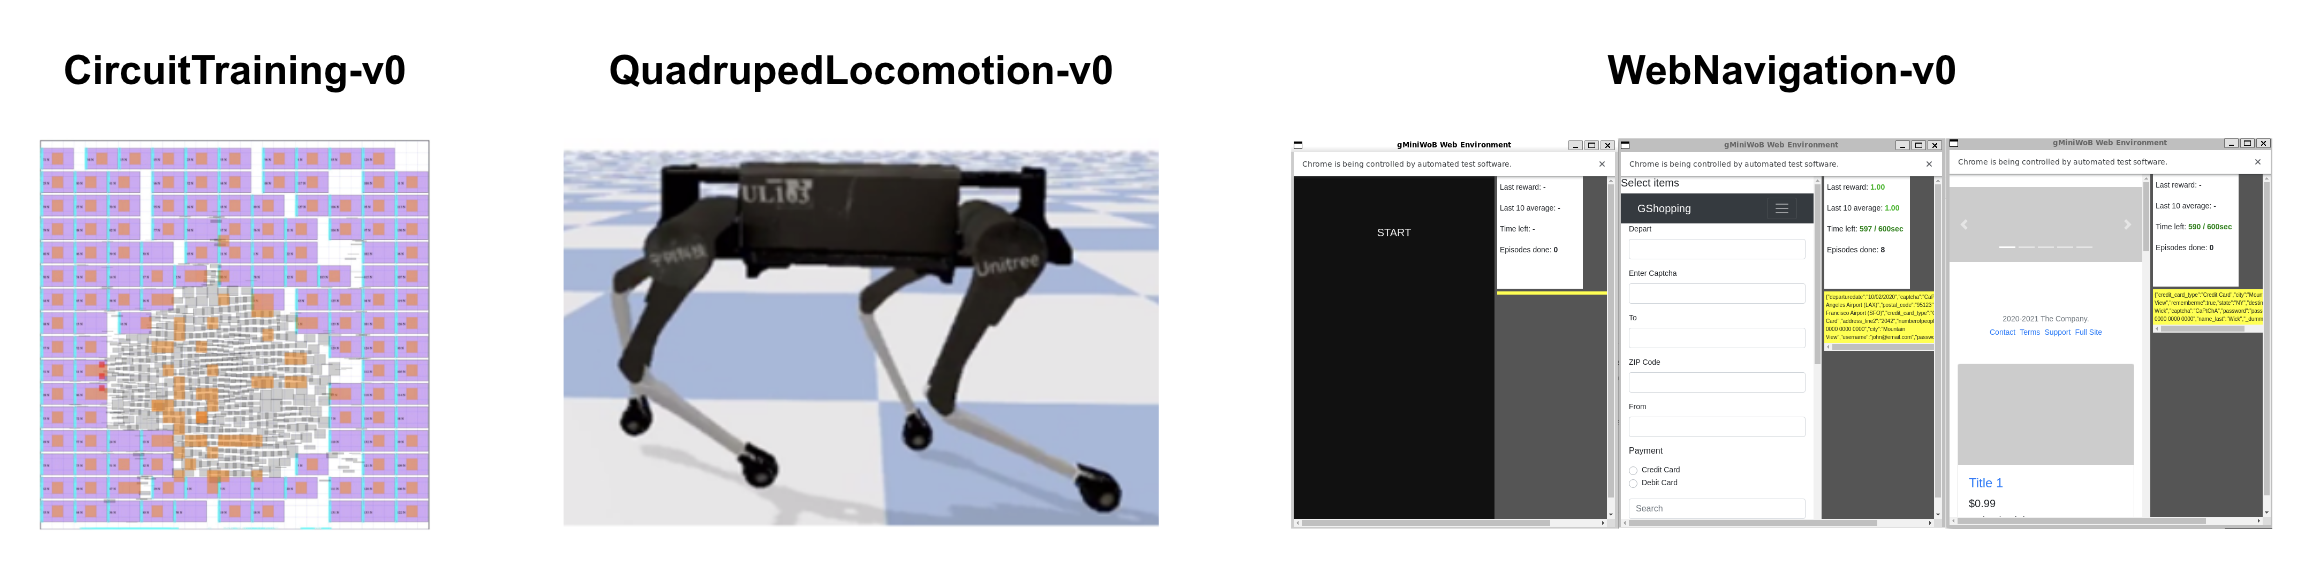
\includegraphics[width=0.95\linewidth]{img/a2perf_envs2.png}
    \caption{The three domains included in A2Perf: computer chip floorplanning for optimizing integrated circuit layouts, web navigation for automated form filling and website interaction, and quadruped locomotion for robotic control. These specific domains were selected based on their demonstrated transfer from simulation to real-world applications.}
    \label{fig:a2perf-domains}
\end{figure}

Our experimental evaluation yields valuable insights into the real-world applicability of autonomous agents across diverse domains.
In the web navigation domain, we explore the feasibility of deploying agents by analyzing their inference time, power usage, and memory consumption, demonstrating that trained agents can operate with latencies comparable to human reaction times on consumer-grade hardware. Furthermore, the reliability metrics \citep{chan2019measuring} prove crucial in selecting agents for chip floorplanning and quadruped locomotion tasks.
For chip floorplanning, we find that the PPO \citep{schulman2017proximal} algorithm provides more consistent initial placements compared to DDQN \citep{van2015ddqn}, reducing variability for designers.
In quadruped locomotion, PPO exhibits superior stability during training, while SAC \citep{haarnoja2018soft_actor_critic} demonstrates more consistent gaits during deployment, highlighting the importance of considering reliability in real-world scenarios.
These findings underscore A2Perf's ability to provide a comprehensive evaluation of autonomous agents, facilitating their successful deployment in practical applications.

